\pagebreak

\addcontentsline{toc}{section}{Введение}
\section*{Введение}
В настоящее время, в период пандемии, люди вынуждены проводить
дома большую часть своего времени. Известно, что мелкие домашние
животные, как, например, кошки, способны уменьшить эффект
изоляции от социума, воспитать в людях доброту и другие положительные качества.
К сожалению, некоторые люди подходят к выбору домашнего животного безответственно,
из-за чего страдает как человек, так и животное.

Кошки дрессируются сложнее собак, они более независимые и их
поведение может определяться не столько воспитанием,
сколько некоторым присущим породе характеристикам.
Среди задач веб-приложения можно выделить:
\begin{itemize}
    \item Отображение списка пород кошек, взятого из публичных
    источников.
    \item Возможность прочитать описание отдельной породы, ее историю,
    особенности здоровья и некоторую другую справочную информацию.
    \item Возможность фильтровать породы кошек некоторым
    характеристикам, например, дружественность к детям, привязанность к семье и т.д.
\end{itemize}

Для решения данных задач было разработано веб-приложение на стеке
React + Spring с использованием Memcached в качестве основного интсрумента СУБД.

\pagebreak
\addcontentsline{toc}{section}{Качественные требования к решению}
\section*{1. Качественные требования к решению}
Разработанное решение должно обладать следующими свойствами/решать следующие задачи:
\begin{itemize}
    \item В качестве СУБД используется Memcached
    \item Существует возможность импорта и экспорта БД
    \item В приложении можно осуществлять фильтрацию пород по численным характеристикам
    \item Приложение может быть развернуто средствами контейнеризации и оркестрации
\end{itemize}

\pagebreak
\addcontentsline{toc}{section}{Сценарии использования}
\section*{2. Cценарии использования}

\addcontentsline{toc}{subsection}{Макет пользовательского интерфейса}
\subsection*{2.1. Макет пользовательского интерфейса}
Общий вид макета пользовательского интерфейса представлен на рисунке 1.
\begin{figure}[H]
    \centering
    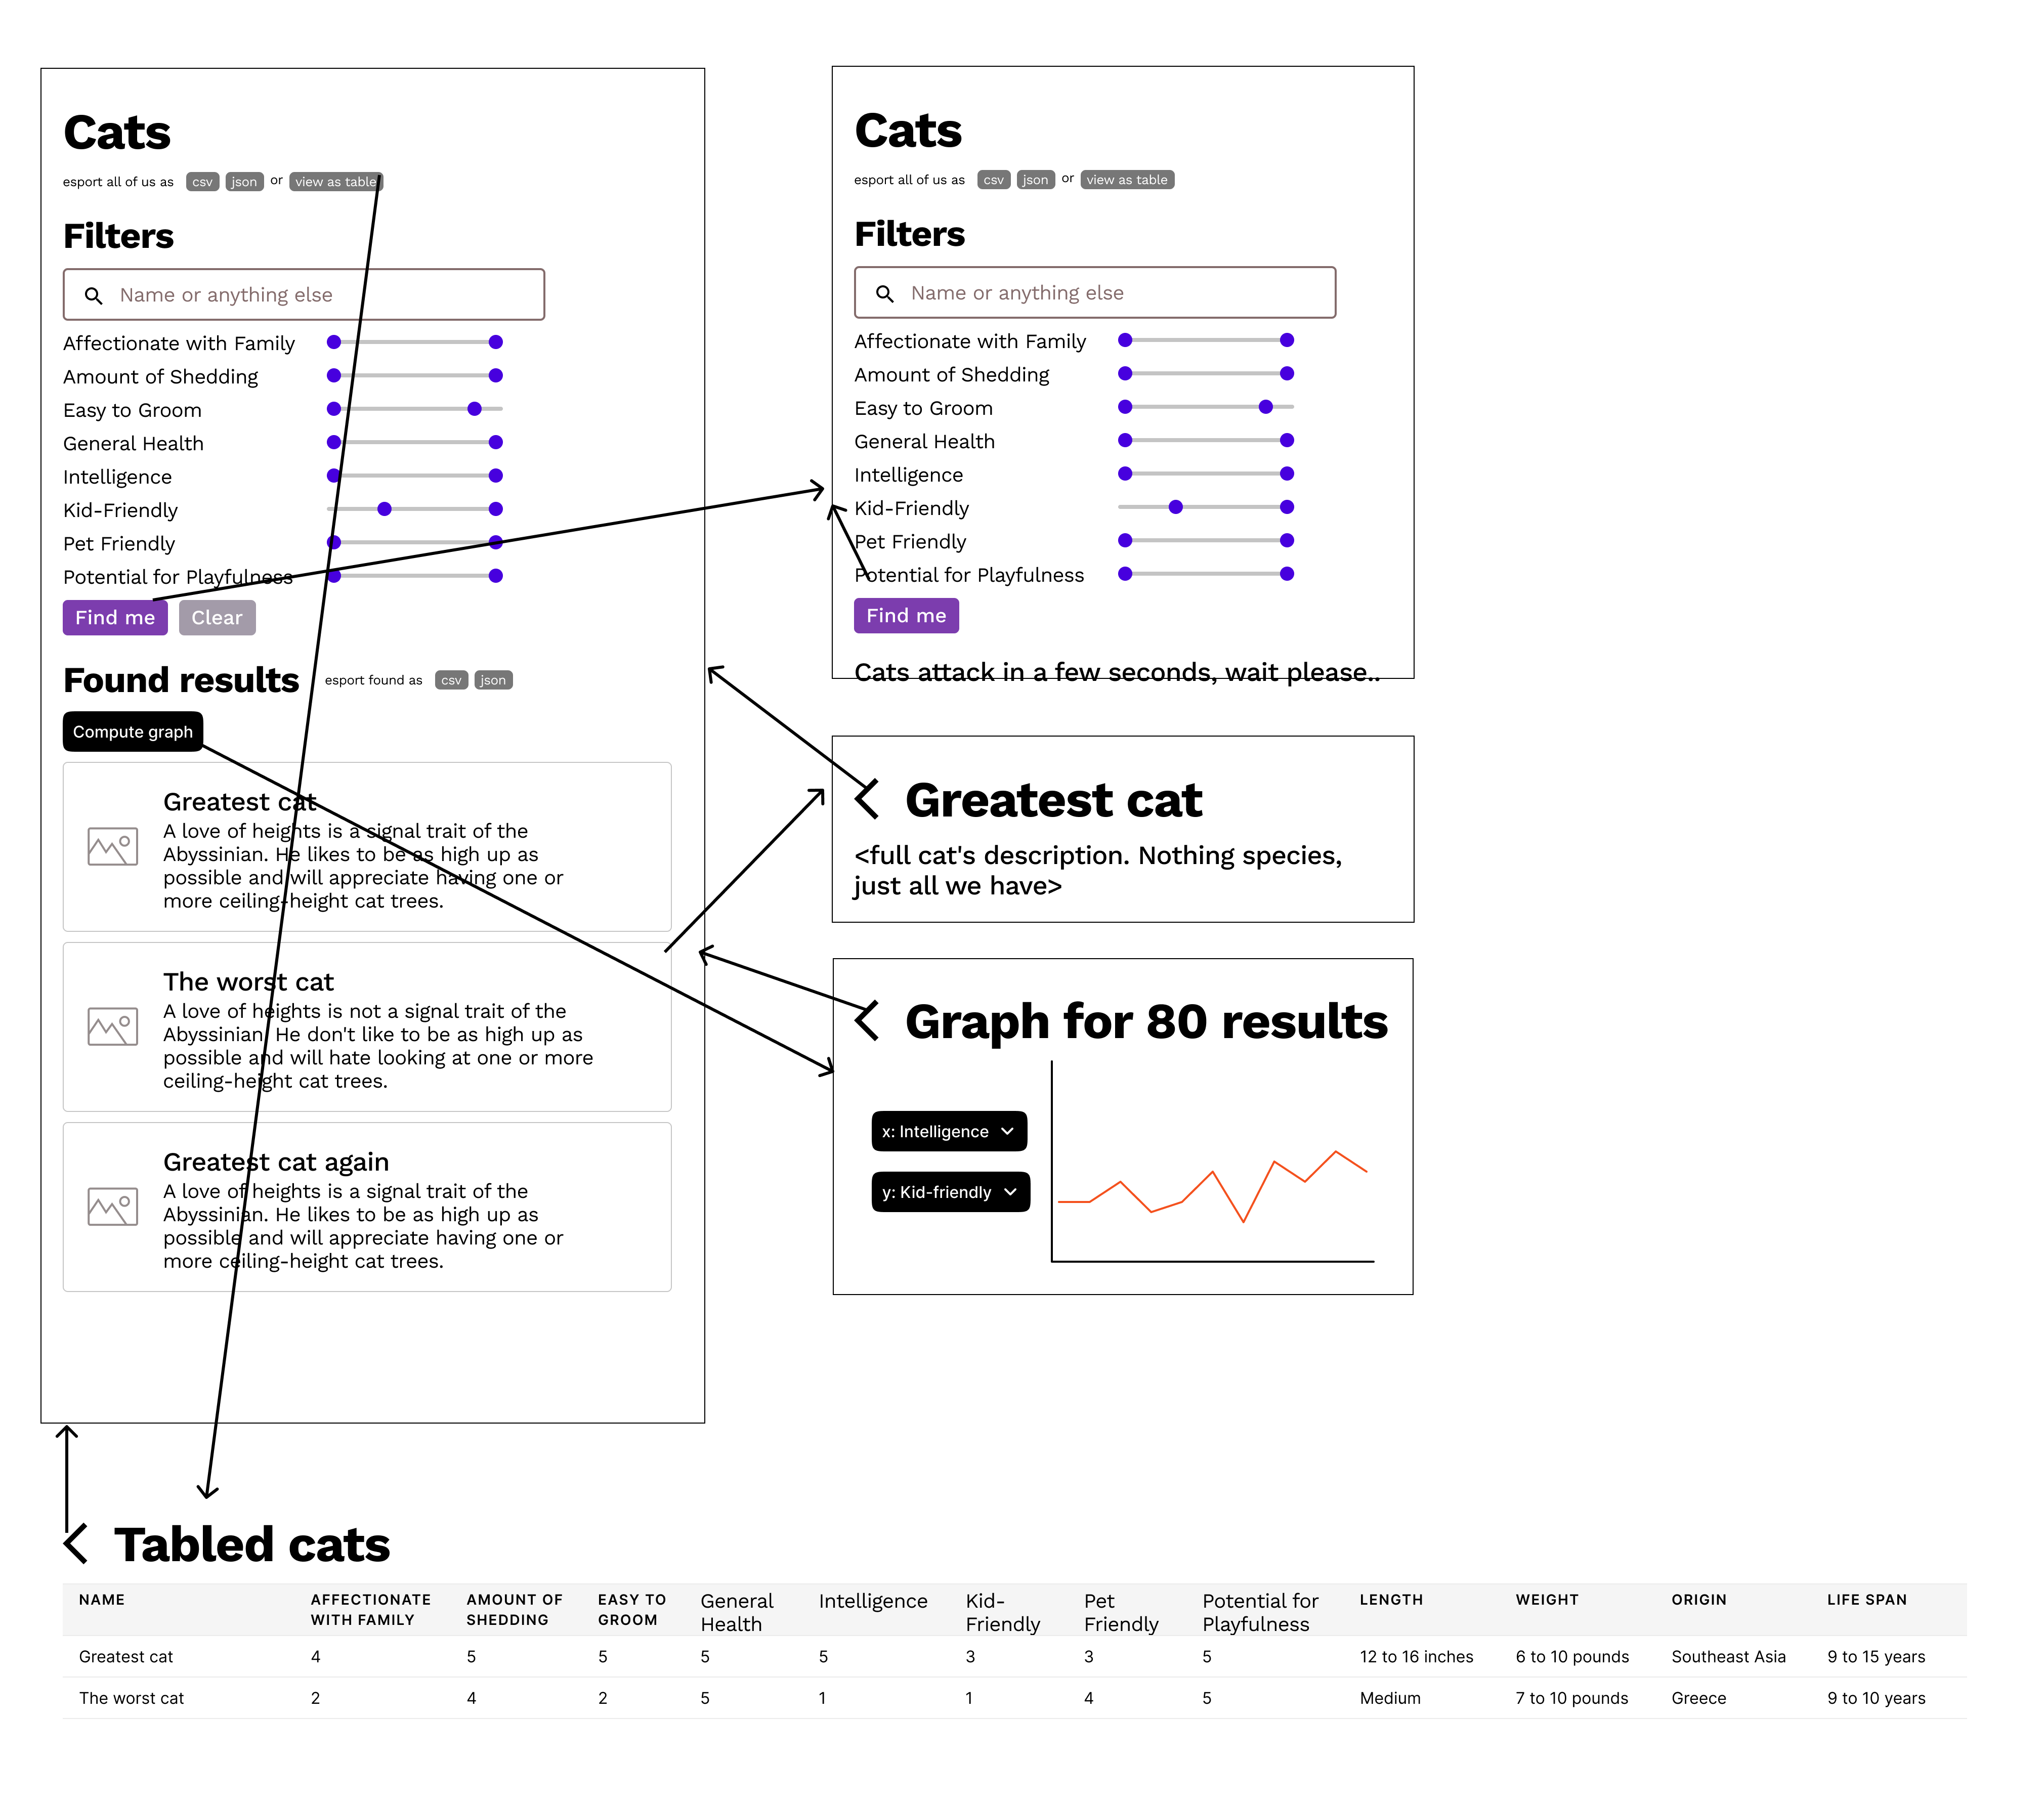
\includegraphics[width=0.9\linewidth]{1}
    \caption*{Рисунок 1 -- Макет пользовательского интерфейса}
    \label{fig:1}
\end{figure}

\addcontentsline{toc}{subsection}{Основные сценарии использования}
\subsection*{2.2. Основные сценарии использования}
\textbf{Фильтрация}
\begin{enumerate}
    \item Пользователь открывает главную страницу.
    \item Пользователь выбирает нужные фильтры: строка поиска и числовые фильтры.
    \item Пользователь нажимает кнопку "Find".
    \item В список ниже загружаются найденные результаты в виде карточек.
\end{enumerate}

\textbf{Открытие детальной информации о коте}
\begin{enumerate}
    \item Возможны 3 варианта:
    \begin{itemize}
        \item Пользователь открывает главную страницу и в списке котов нажимает на желаемую карточку.
        \item Пользователь вводит в адресную строку ссылку на интересующего его кота.
        \item Пользователь открывает просмотр всех данных в виде таблицы и выбирает интересующею его строку.
    \end{itemize}
    \item Открывается страница с детальной информацией о коте.
\end{enumerate}

\textbf{Просмотр графика зависимости одного параметра от другого}
\begin{enumerate}
    \item Пользователь заходит на главную страницу.
    \item Опционально. Пользователь фильтрует данные (см п. Фильтрация).
    \item Пользователь нажимает кнопку "Compute graph".
    \item Открывается страница с графиком для найденных результатов.
    \item На графике пользователь выбирает из выпадающего списка поля по оси X и по оси Y.
    \item Строится график зависимости поля Y от поля X. Для каждого значения X находятся коты с соответствующим значением и среди них считается среднее Y, которое берется как Y значение точки на графике.
\end{enumerate}

\textbf{Экспорт найденных результатов}
\begin{enumerate}
    \item Пользователь заходит на главную страницу.
    \item Опционально. Пользователь фильтрует данные.
    \item Пользователь в разделе экспорта выбирает формат экспорта и нажимает на кнопку.
    \item Выполняется экспорт данных путем переадресации на страницу, где на сервере формируется ответ в виде файла.
\end{enumerate}

\textbf{Экспорт всех данных базы}
\begin{enumerate}
    \item Пользователь заходит на главную страницу.
    \item Пользователь в разделе экспорта всех данных выбирает тип экспорта.
    \item Выполняется экспорт данных путем переадресации на страницу, где на сервере формируется ответ в виде файла.
\end{enumerate}

\textbf{Просмотр содержимого базы в виде таблицы}
\begin{enumerate}
    \item Пользователь заходит на главную страницу.
    \item Пользователь в разделе экспорта всех данных выбирает "View as a table".
    \item Открывается страница с данными базы, представленными в виде таблицы. В ней отображены только те поля, которые можно кратко записать в ячейки (длинные описания опущены).
\end{enumerate}

\addcontentsline{toc}{subsection}{Вывод}
\subsection*{2.3. Вывод}
На основании рассмотренных сценариев использования было выявлено,
что основные операции при взаимодействии пользователей с приложением --
операции чтения.

\pagebreak
\addcontentsline{toc}{section}{Модель данных}
\section*{3. Модель данных}
\addcontentsline{toc}{subsection}{Схема данных}
\subsection*{3.1. Схема данных}
В приложении используется единственная сущность -- Порода кошки.

Порода описывается следующими свойствами

\noindent\textit{Таблица 1 -- Описание свойств породы}
\begin{longtable}{|p{7.5cm}|p{7.5cm}|}
    \hline
    \textbf{Название свойства}       & \textbf{Описание}                                  \\\hline
    Название породы                  & Строка, может быть использована как первичный ключ \\\hline
    Привязанность к семье            & Число от 0 до 5                                    \\\hline
    Склонность к линьке              & Число от 0 до 5                                    \\\hline
    Простота ухода                   & Число от 0 до 5                                    \\\hline
    Доброжелательность к незнакомцам & Число от 0 до 5                                    \\\hline
    Общее здоровье                   & Число от 0 до 5                                    \\\hline
    Общий интеллект                  & Число от 0 до 5                                    \\\hline
    Доброжелательность к детям       & Число от 0 до 5                                    \\\hline
    Доброжелательность к животным    & Число от 0 до 5                                    \\\hline
    Игривость                        & Число от 0 до 5                                    \\\hline
    Склонность к пению               & Число от 0 до 5                                    \\\hline
    Длина                            & Строка, пример "Medium"                            \\\hline
    Продолжительность жизни          & Строка, пример "12 to 16 years"                    \\\hline
    Регион происхождения             & Строка, пример "California, USA"                   \\\hline
    Вес                              & Строка, пример "5 to 10 pounds"                    \\\hline
    Информация об уходе              & Текст                                              \\\hline
    Дети и животные                  & Текст                                              \\\hline
    Цвет и уход                      & Текст                                              \\\hline
    Здоровье                         & Текст                                              \\\hline
    История породы                   & Текст                                              \\\hline
    Характер                         & Текст                                              \\\hline
    Короткое описание                & Текст                                              \\\hline
    Изображение                      & Ссылка                                             \\\hline
    Размер                           & Текст                                              \\\hline
\end{longtable}

Список пород кошек -- почти постоянный, в том смысле, что может быть занесен в программу один раз и будет изменяться
крайне редко. Основными запросами к приложению будут \textbf{получение} полной информации о каждой породе и \textbf{фильтрация}
списка пород по заданным параметрам (например, по уровню интеллекта или продолжительности жизни).

Исходя из этого будет выбираться модель представления, в которой упомянутые операции будут выполняться быстрее других
(изменение, добавление, удаление).

\addcontentsline{toc}{subsection}{Нереляционная модель данных}
\subsection*{3.2. Нереляционная модель данных}
В качестве нереляционной БД в приложении используется Memcached. Memcached позволяет хранить отображения вида
строка-строка (грубо Map<String, String>), не имеет поддержки конкурентности, транзакционности и прочих прелестей, что
накладывает серьезные ограничения на способ представления данных.

Также упомянем, что задание включает в себя требование о том, что некоторые операции над данными должны совершаться
средствами используемой БД, что тяжело себе вообразить с таким инструментом, как Memcached.

Исходя из ограничений используемого инструмента и требований к быстродействию операций, положим следующую
модель.

Будем хранить 3 типа отображений: all\_cats, \{ breed\_name \}.\{ characteristic\_name \}
, \{ vital\_stat / characteristic\_name \}.\{ vital\_stat\_value / characteristic\_value \}.

Первое отображение специальное, имеет зарезервированный ключ и позволяет получить строку со списком всех названий пород.

Отображения вида \{ breed\_name \}.\{ characteristic\_name \} позволяют хранить свойства породы. Например, Abyssinian.health
содержит "Both pedigreed cats and mixed-breed cats have varying incidences...".

Отображения вида \{ vital\_stat / characteristic\_name \}.\{ vital\_stat\_value / characteristic\_value \} хранят список пород,
удовлетворяющих заданным характеристикам. Например, length.Medium или intelligence.4 содержит Abyssinian и др.

Отображение первого типа позволяет поддерживать список первичных ключей.

Отображения второго типа позволяют связывать первичный ключ записи с остальными полями.

Отображения третьего типа позволяют оптимизировать процесс фильтрации по характеристикам.

Графически модель приведена на рисунке 2.
\begin{figure}[H]
    \centering
    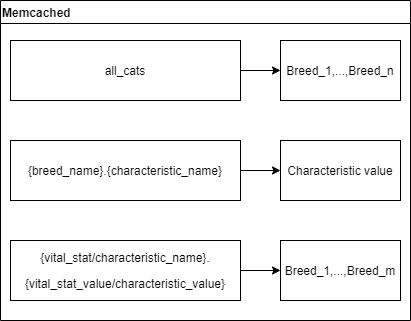
\includegraphics[width=0.9\linewidth]{2}
    \caption*{Рисунок 2 -- Модель данных в Memcached}
    \label{fig:2}
\end{figure}

\addcontentsline{toc}{subsection}{Оценка удельного объема информации, нереляционная модель}
\subsection*{3.3. Оценка удельного объема информации, нереляционная модель}

Размер символа определяется клиентской стороной. Примем его равным 2 байтам.

Пусть $N$ -- количество пород в базе.

Тогда отображение первого типа будет занимать 8 ("all\_cats") + (N-1)(,) + N * BNAME\_SIZE. Приняв верхнюю оценку для
BNAME\_SIZE равную 20 символов получим примерно 21N символов.

Отображения второго типа разделим на два вида: значения представленные числом или короткой строкой (до 30 символов) и
значения, содержащие текст с длиной больше 30 символов.

Рассмотрим первый вид. Размер ключа BNAME\_SIZE + 1 (.) + CNAME\_SIZE = 46, при выборе CNAME\_SIZE в качестве 25 символов.
25 символов -- длина "Potential for Playfulness". Значения первого вида -- числа или короткие строки, например, 4 или "
Quebec, Canada", их размер оценим в 30 символов. Для каждой кошки имеется 14 характеристик подобного вида,
получаем N * (46 + 30) * 14 = 1064N символов. Это верхняя оценка.

Рассмотрим второй вид. Размер ключа BNAME\_SIZE + 1 (.) + CNAME1\_SIZE = 36, при выборе CNAME1\_SIZE в качестве 15
символов. Для каждой кошки имеется 9 характеристик с текстом (url-картинки отнесем к этому виду), размер текста в
среднем для каждой характеристики кошки примем равным 1000 символов. Получаем оценку N * (36 * 9 + 9 * 1000) = 9324N
символов.

Итого для отображения второго типа 1064N + 9324N = 10388N символов.

Рассмотрим отображения третьего типа. Размер ключа CNAME\_SIZE + 1 (.) + CHAR\_VAL\_LENGTH = 56, CHAR\_VAL\_LENGTH = 30
символов. Для численных значений характеристик имеем 6 * 10 * KEY\_SIZE + N * BNAME\_SIZE = 3360 + 20N, так как у каждой
кошки есть значение численное значение характеристики и только одно. Со строковыми характеристиками сложнее, они очень
сильно варьируются, поэтому дадим грубую оценку в M * KEY\_SIZE + N * BNAME\_SIZE = N * 56 + 20N = 76N, где в качестве M
было взято N -- все значения различны. В реальных данных есть пересечения и размер модели будет меньше.

Итого получаем верхнюю оценку 21N + 10388N + (76N + 20N + 3360) = 10505N + 3360.
Или 21010N + 6720 байтов.

Рост происходит линейным образом.

\addcontentsline{toc}{subsection}{Избыточность нереляционной модели}
\subsection*{3.4. Избыточность нереляционной модели}

Для каждой характеристики имеем избыточность в виде повторного хранения названии породы для маппинга и хранения названия
характеристики. Избыточность этого вида можно оценить
как N * (14 * (CNAME\_SIZE + BNAME\_SIZE + 1) + 9 * (CNAME1\_SIZE + BNAME\_SIZE + 1)) = 968N.

Также все отображения третьего типа избыточны, они используются в поиске/фильтрации, их размер равен 96N + 3360.

Общую избыточность можно оценить как 1064N + 3360.

Для оценки избыточности получаем формулу (10505N + 3360) / (9441N). В пределе для выражения для избыточности получаем
значение 1.112.

\addcontentsline{toc}{subsection}{Запросы к нереляционной СУБД}
\subsection*{3.5. Запросы к нереляционной СУБД}
Запросы к Memcached имеют вид {get/add/remove} key и не представляют особого интереса.

Оценим количество запросов к БД для \textit{CRUD} операций.

\textbf{Добавление}

Пусть нужно сохранить одну кошку породы Barsik. Тогда нужно прочитать кортеж по ключу all\_cats, добавить в него
строку Barsik и сохранить обратно. Получим 2 операции с базой. Количество ключей не изменится.

Затем для каждой строковой характеристики, которых может быть 9, нужно добавить
запись Barsik.{ characteristic\_name } = { characteristic\_value }. Еще 9 операций и столько же новых ключей.

Добавление составных характеристик.
\begin{itemize}
    \item Во-первых, имеется 10 числовых характеристик, которые могут принимать 6 значений, но в случае с добавлением одной
  кошки нужно создать 10 новых пар ключ-значение или добавить в существующий кортеж 10 значений. Получим 20 операций с
  базой и 10 новых ключей.
    \item Во-вторых, есть 4 характеристики, значения которых пересекаются, но не очень часто, поэтому зачастую придется
  создавать новые пары, а не модифицировать существующие. Еще 6 операций и 4 новых ключа. Если кошек 50, то ключей в
  конечном итоге будет примерно 200.
\end{itemize}

Подводя итог, добавление в базу одной кошки требует 37 операций и 23 новых ключа. При 50 кошках получим 1850 операций и
1150 ключей. Выглядит максимально не оптимально, но таковы ограничения используемой базы.

\textbf{Чтение}

Рассмотрим чтение кошек отфильтрованных по какому-либо парамеру. Чтобы получить список пород удовлетворяющих параметру,
нужно сделать всего один запрос. Но чтобы восстановить кошку, то есть собрать все поля из базы, нужно сделать:

\begin{itemize}
    \item 9 запросов для каждой текстовой характеристики;
    \item 14 запросов для остальных характеристик;
\end{itemize}

Имеем 25 запросов в базу.

Чтение JSON сериализованной кошечки и десериализация могли бы выполняться за 1 запрос, но этого могло бы нарушить
ограничения на использования БД (все основные операции должны выполняться средствами БД).

\textbf{Обновление}
\begin{itemize}
    \item Если пришлось изменить название породы, то нужно изменить его в кортеже all\_cats, изменить 23 ключа и изменить его
  еще в 260 кортежах, где эта порода потенциально может быть. Итого 545 операций с базой.
    \item Чтобы изменить описательную характеристику, потребуется одна операция.
    \item Если изменяется какая-либо составная характеристика кошки, то нужно удалить кошку из кортежа с прошлой
  характеристикой, и добавить в кортеж с новой характеристикой. Итого 2 операции с базой.
\end{itemize}

\textbf{Удаление}

Удаляется кошка путем удаления названия породы из кортежа all\_cats и еще 260 кортежей с характеристиками, и также
удалится 23 пары ключ-значение. Всего (260 + 1) * 2 + 23 = 545 операции с базой.


\addcontentsline{toc}{subsection}{Реляционная модель данных}
\subsection*{3.6. Реляционная модель данных}
Модель состоит из идентификатора, названия породы, 9 строковых характеристик, 10 числовых характеристик и 4 оставшихся
строковых характеристик.

В качестве SQL решения будем опираться на Postgres.

Графическое представление модели приведено на рисунке 3.

\begin{figure}[H]
    \centering
    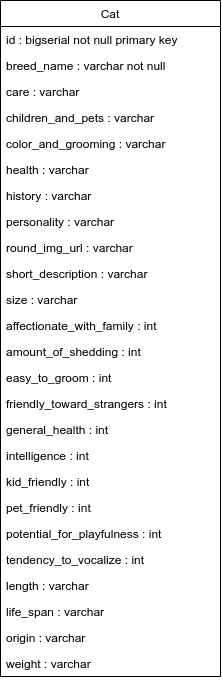
\includegraphics[height=15cm]{3}
    \caption*{Рисунок 3 -- Модель данных в Postgres}
    \label{fig:3}
\end{figure}

\textbf{Оценка удельного объема информации, хранимой в модели}

Пусть в базе лежит $N$ пород, размер символа 2 байта, bigserial - 8, int - 4, тогда размер модели будет равен
N * (8 + 20 + 9 * 1000 * 2 + 10 * 4 + 4 * 30 * 2) = 18308N байтов.

\textbf{Избыточность модели}

В модели нет избыточности.

\addcontentsline{toc}{subsection}{Запросы к реляционной СУБД}
\subsection*{3.7. Запросы к реляционной СУБД}
Для добавления кошки в таблицу нужен 1 запрос:

\begin{lstlisting}
INSERT INTO cat(breed, care, ...)
VALUES (?, ?...);
\end{lstlisting}

При этом в таблицу добавится только 1 строка.

Для поиска кошки по любому параметру так же нужен всего 1 запрос:

\begin{lstlisting}
SELECT *
FROM cat
WHERE param1 = ? AND param2 = ?
   OR param3 > ?;
\end{lstlisting}

Для обновления информации о кошке нужен вновь всего 1 запрос:

\begin{lstlisting}
UPDATE cat
SET param1=?, ....
    WHERE id=?;
\end{lstlisting}

Для удаления кошки так же 1 запрос:

\begin{lstlisting}
DELETE
*
FROM cat
WHERE id = ?;
\end{lstlisting}

\addcontentsline{toc}{subsection}{Выводы}
\subsection*{3.8. Выводы}
Для нереляционной модели была получена оценка 21010N + 6720 байтов, где $N$ -- количество пород.
Это оценка сверху, в ней принято допущение, что текстовые характеристики занимают 1000 символов, хотя они практически
все меньше.
Memcached позволяет хранить их без необходимости дополнения до 1000 символов.
С другой стороны, модель имеет избыточные данные, используемые для маппинга ключа на свойства и вспомогательные отображения
для фильтрации.

Для реляционной модели была получена оценка 18308N байтов, данные хранятся без избыточности в одной таблице.

В обоих случаях объем данных растет линейно относительно количества пород.

При анализе количества запросов все встает на свои места.

Для выполнения необходимых функций в реляционной модели достаточно 1 запроса для каждого действия.
В нереляционной модели для выполнения тех же операций необходимо поддерживать весьма специфические отображения,
сложнее поддерживать согласованность данных, количество запросов неприлично большое даже для простейших CRUD операций.

В данной задаче совершенно неоправданно использование Memcached в качестве БД, как и во всех случаях его использования
не по назначению.
Memcached стоит использовать для кэширования примитивных значений, сериализованных объектов, но никак не для моделирования
более сложных структур, требующих дополнительной логики.

\pagebreak
\addcontentsline{toc}{section}{Разработанное приложение}
\section*{4. Разработанное приложение}
\addcontentsline{toc}{subsection}{Краткое описание}
\subsection*{4.1. Краткое описание}
Главная страница приложения выглядит следующим образом (см. рис. 4).
\begin{figure}[H]
    \centering
    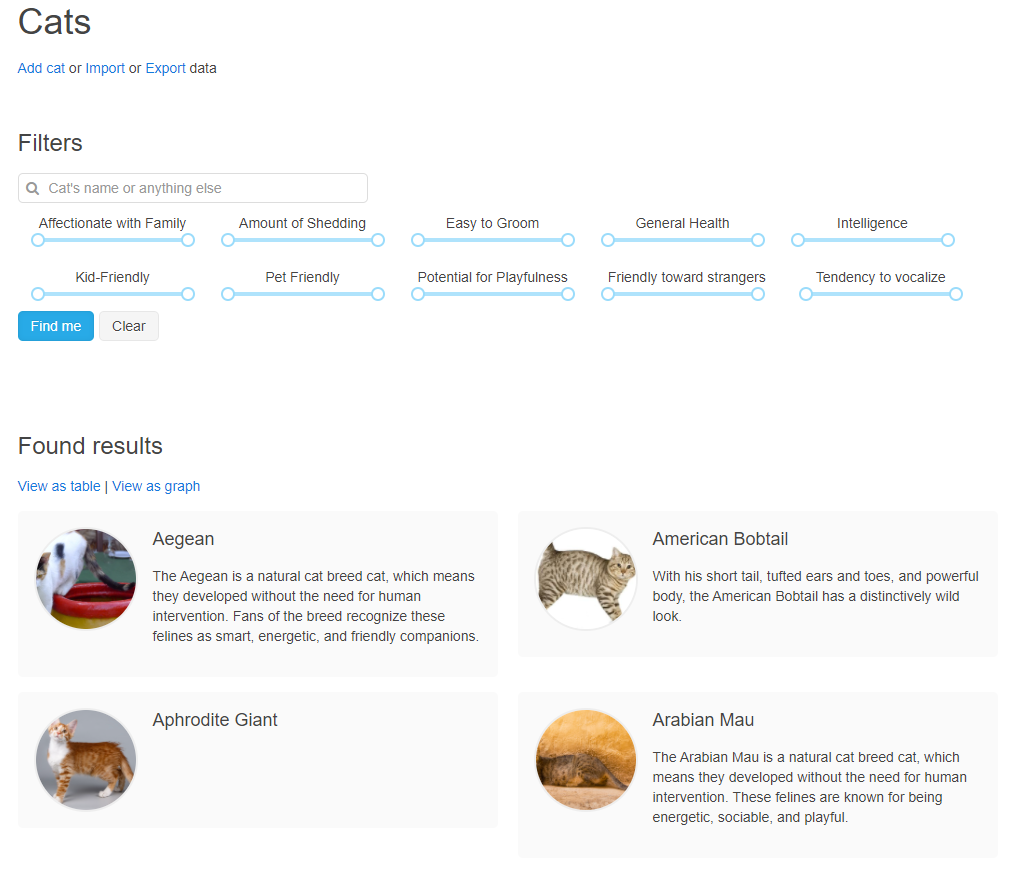
\includegraphics[width=0.9\linewidth]{4}
    \caption*{Рисунок 4 -- Главная страница}
    \label{fig:4}
\end{figure}

Существует возможность поиска породы по названию (см. рис. 5).
\begin{figure}[H]
    \centering
    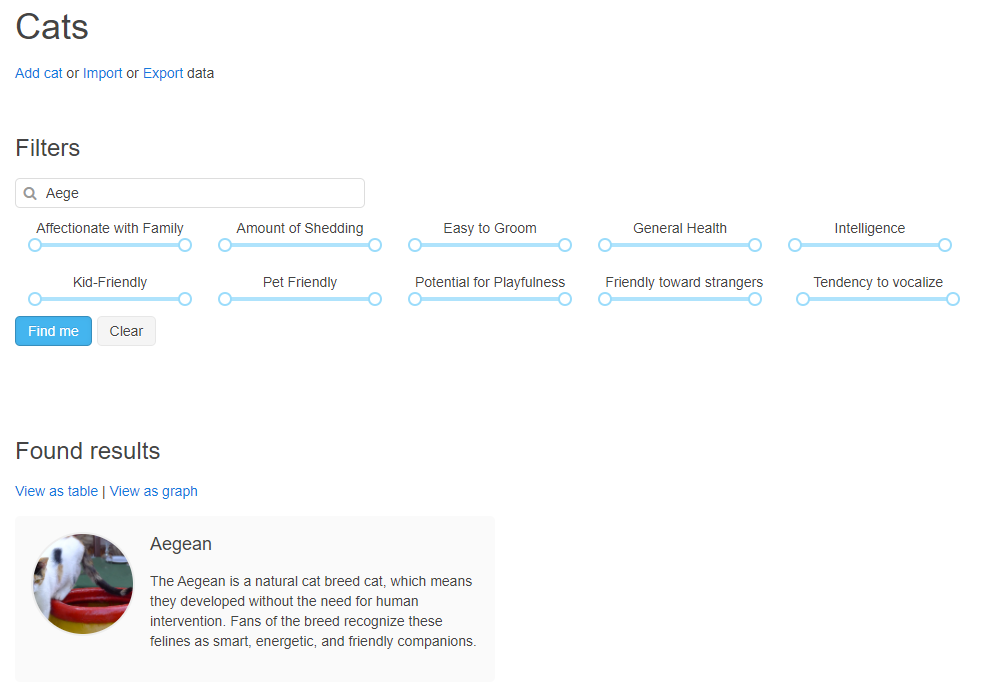
\includegraphics[width=0.9\linewidth]{5}
    \caption*{Рисунок 5 -- Поиск породы по названию}
    \label{fig:5}
\end{figure}

Давайте выберем самых умных и ласковых с семьей кошек (см. рис. 6).
\begin{figure}[H]
    \centering
    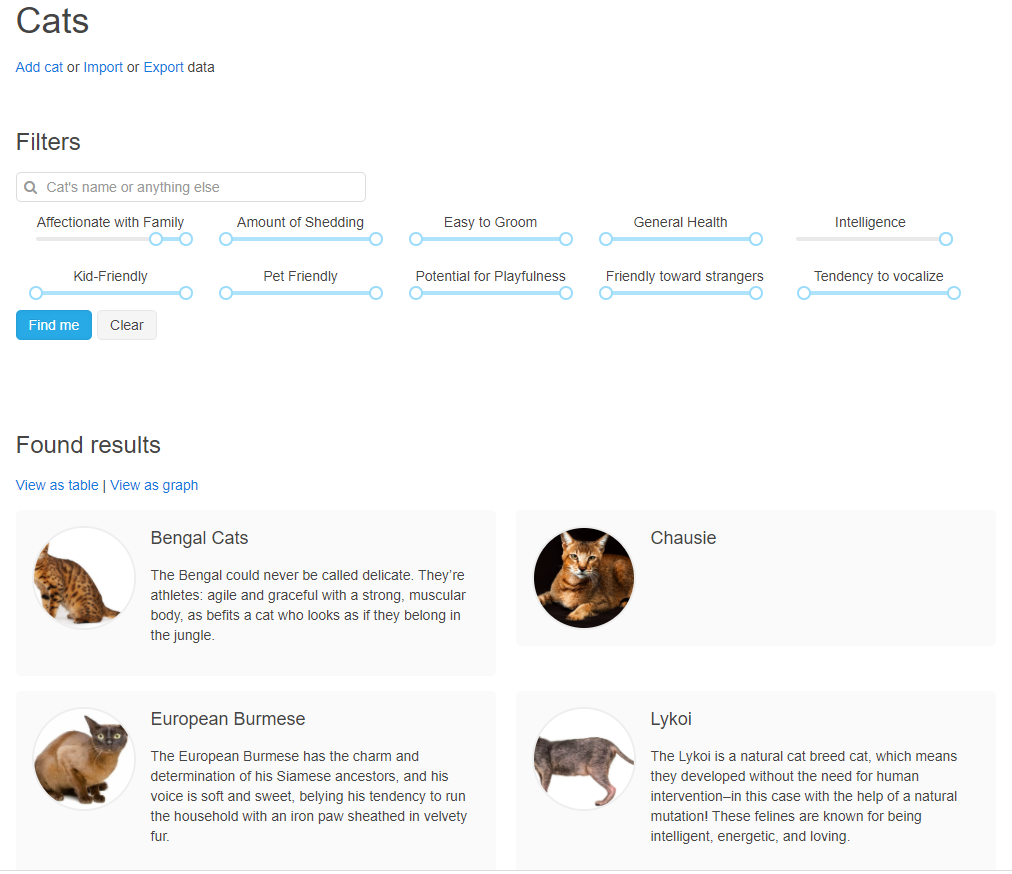
\includegraphics[width=0.9\linewidth]{6}
    \caption*{Рисунок 6 -- Фильтрация пород по характеристикам}
    \label{fig:6}
\end{figure}

Список пород можно представить в виде таблицы (см. рис. 7).
\begin{figure}[H]
    \centering
    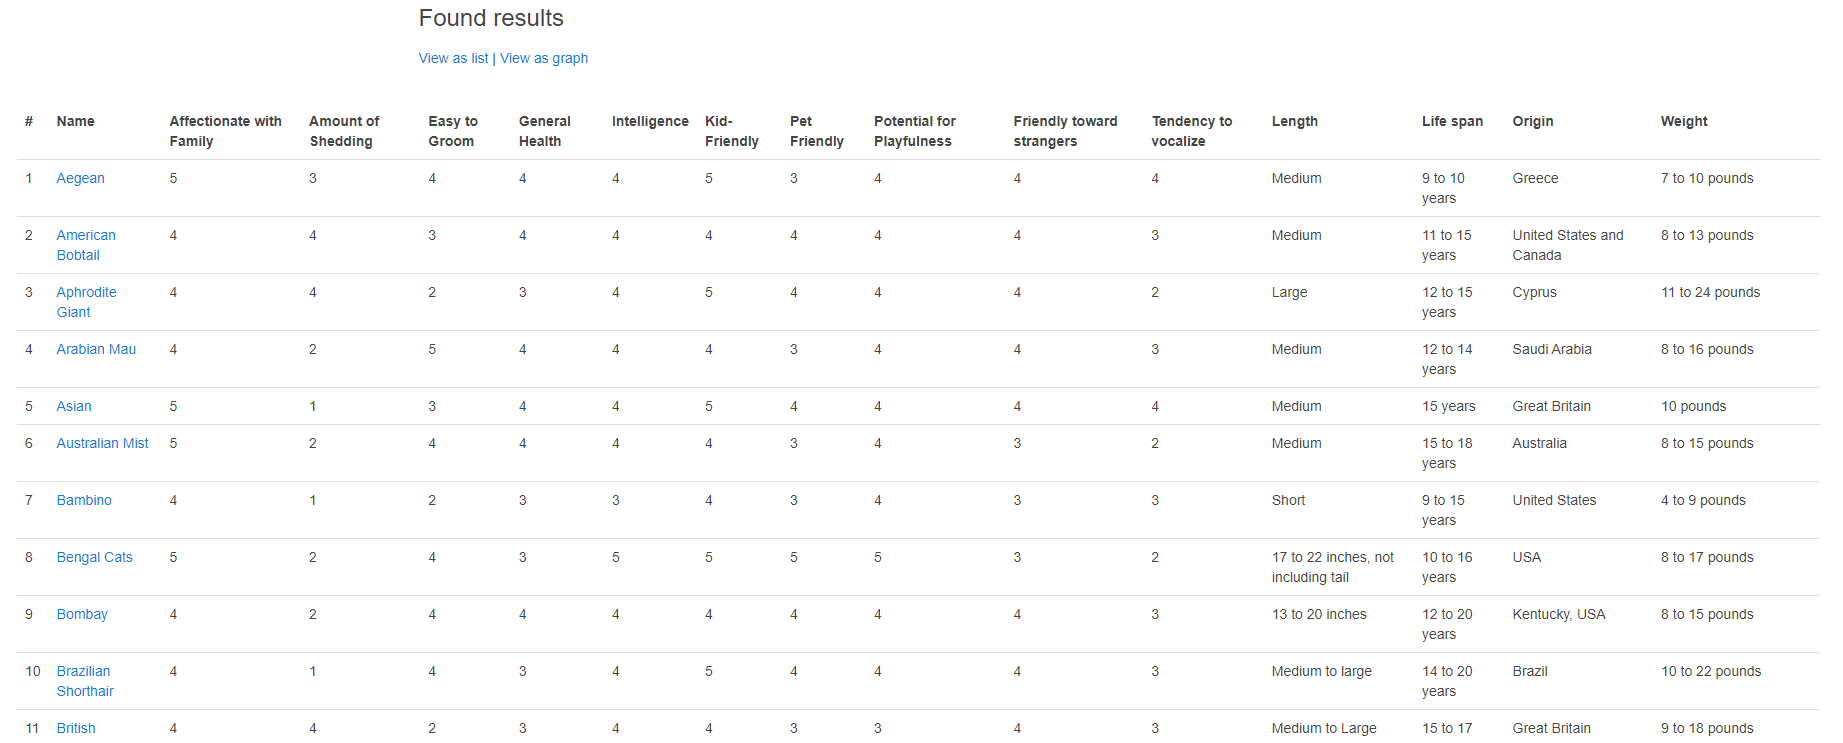
\includegraphics[width=0.9\linewidth]{7}
    \caption*{Рисунок 7 -- Представление пород в виде таблицы}
    \label{fig:7}
\end{figure}

Существует возможность просмотра графика для выборки для двух характеристик.
\begin{figure}[H]
    \centering
    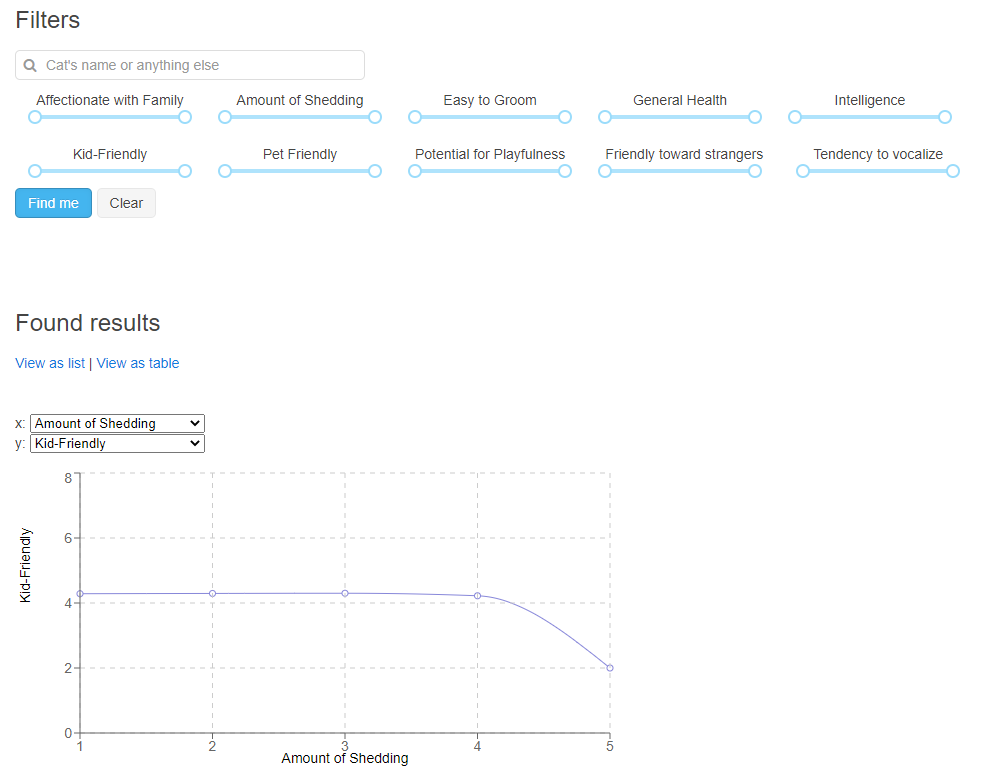
\includegraphics[width=0.9\linewidth]{8}
    \caption*{Рисунок 8 -- График характеристик}
    \label{fig:8}
\end{figure}

Полученный график следует интерпретировать так: для кошек с характеристикой
Amount of Shedding среднее Kid-Friendly равно 2.

Каждую породу можно рассмотреть отдельно в формате карточки (см. рис. 9).
\begin{figure}[H]
    \centering
    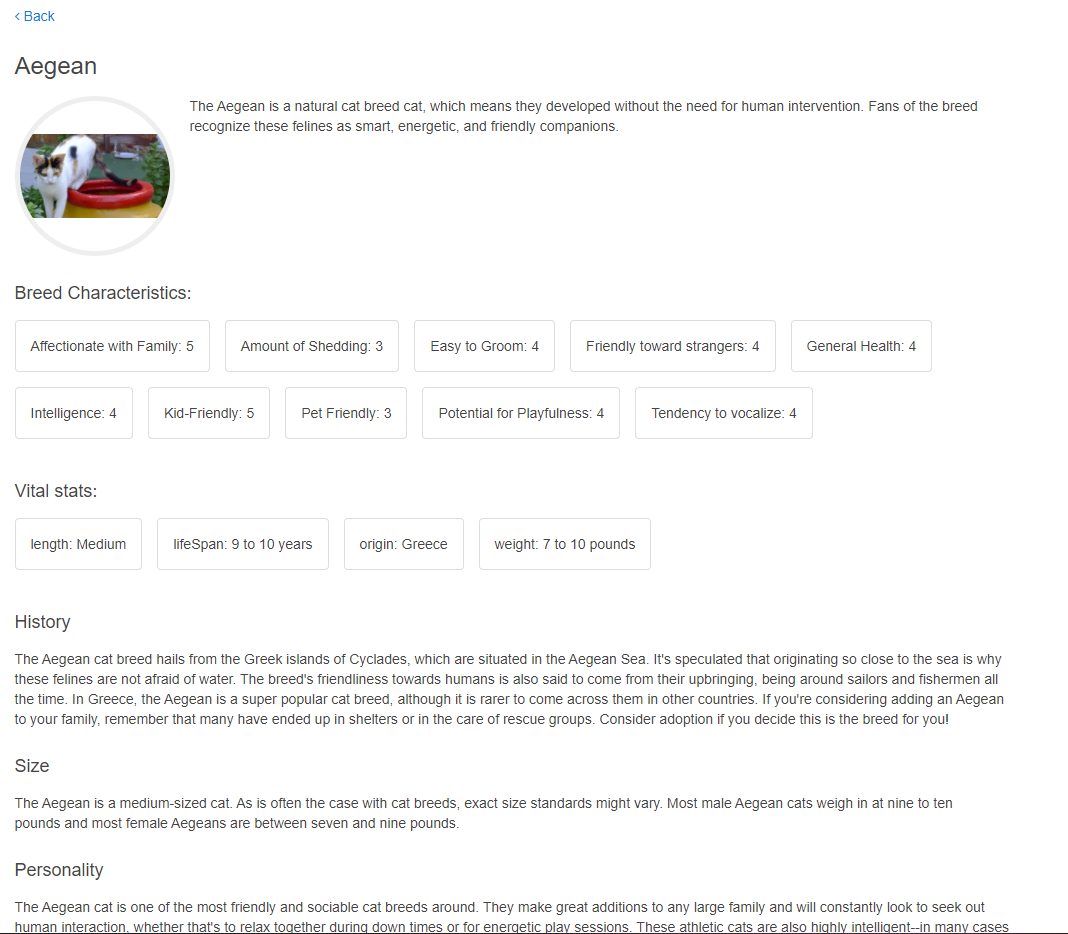
\includegraphics[width=0.9\linewidth]{9}
    \caption*{Рисунок 9 -- Карточка породы}
    \label{fig:9}
\end{figure}

Для импорта данных имеется простенькая форма (см. рис. 10).
\begin{figure}[H]
    \centering
    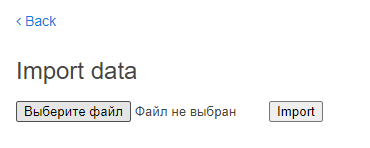
\includegraphics[width=0.9\linewidth]{10}
    \caption*{Рисунок 10 -- Форма для импорта}
    \label{fig:10}
\end{figure}

\pagebreak
\addcontentsline{toc}{section}{Экспериментальная проверка теоретических оценок для Memcached}
\section*{5. Экспериментальная проверка теоретических оценок для Memcached}
Зависимость фактического объема хранимых данных от количества пород приведена на рисунке 11.
По оси X отложено количество пород, по оси Y количество занимаемого пространства в байтах.
\begin{figure}[H]
    \centering
    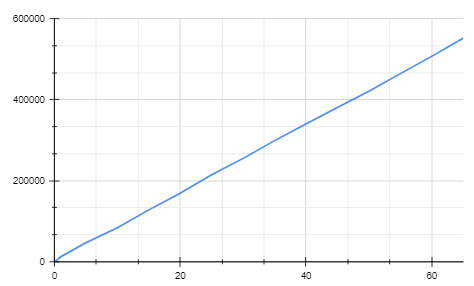
\includegraphics[width=0.9\linewidth]{11}
    \caption*{Рисунок 11 -- Зависимость объема данных от числа пород}
    \label{fig:11}
\end{figure}

Теоретическая оценка асимптотика оказалась верной.

С временем выполнения операций немного сложнее.
Существует некоторое постоянное время необходимое на установление соединения, время
некоторой обработки данных, например, установка полей data transfer object.
На рисунке 12 приведена завимость времени выполнения операции от количества уже имеющихся
пород в БД.
По оси X отложено количество кошек в БД, по оси Y время в секундах
\begin{figure}[H]
    \centering
    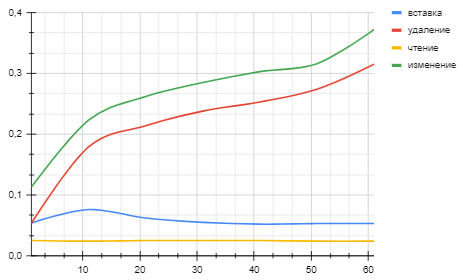
\includegraphics[width=0.9\linewidth]{12}
    \caption*{Рисунок 12 -- Зависимость времени работы от числа пород}
    \label{fig:12}
\end{figure}

Стоит отметить, что пород кошек в мире существует не так много, поэтому решение не обязано
масштабироваться на объем больший $10^3$.
По графику можно определить, что чтение данных занимает константное время.
Операции удаления и изменения наиболее затратные, как и ожидалось в теоретическом анализе.

\pagebreak
\addcontentsline{toc}{section}{Заключение}
\section*{Заключение}
В результате выполнения курсового проекта было разработано приложение для
поиска и фильтрации пород кошек по некоторым характеристикам.
Приложение позволяет:
\begin{itemize}
    \item Просмотреть список пород кошек, взятый из известных источников
    \item Отфильтровать породы по некоторым желаемым характеристикам
    \item Импортировать и экспортировать данные
    \item Получить справочную информацию о породе
\end{itemize}

Дальнейшие шаги для улучшения решения:

\begin{itemize}
    \item Использовать реляционную СУБД в качестве основной СУБД, а Memcached по его назначению
    как вспомогательный инструмент
    \item Для каждой породы добавить галерию с фотографиями
    \item Использовать больше публичных источников для сбора и корректировки данных
\end{itemize}

\pagebreak
\addcontentsline{toc}{section}{Приложения}
\section*{Приложения}
\addcontentsline{toc}{subsection}{Сборка и развертывание приложения}
\subsection*{Сборка и развертывание приложения}
\begin{itemize}
    \item Необходимо установить docker и docker-compose
    \item Запустить команду docker-compose up из корня проекта
\end{itemize}